%%%%%%%%%%%%%%%%%%%%%%%%%%%%%%%%%%%%%%%%%%%%%%%%%%%%%%%%%%%%%%%%%%%%
% Authors: A. Herrera-Poyatos, F. Herrera
% Tittle: Algoritmo memético equilibrado con diversificación voraz
% 							 CAEPIA 2015
%%%%%%%%%%%%%%%%%%%%%%%%%%%%%%%%%%%%%%%%%%%%%%%%%%%%%%%%%%%%%%%%%%%%

\section{TPCx-HS}

	\subsection*{¿Por qué usar TPCx-HS?}

		\begin{frame}{Información sobre TPCx-HS}
			\begin{itemize}
				\item Provee de una medida de rendimiento fiable y de rendimiento relación precio.
				\item Permite medir tanto hardware como software y es exclusivo para Hadoop.
			\end{itemize}
			
			\color{ChetwodeBlue}\large Carga de trabajo de TPCx-HS
			
			\begin{itemize}
				\item HSGen: genera los datos según un factor de escala.
				\item HSDataCheck: comprueba el cumplimiento del conjunto de datos.
				\item HSSort: ordena los datos según un orden total.
				\item HSValidate: comprueba si los datos obtenidos son válidos.
			\end{itemize}		
		\end{frame}
	
	\subsection*{Funcionamiento de TPCx-HS}	

		\begin{frame}{Ejecución de TPCx-HS}
				\begin{columns}[c]
					\column{.6\textwidth}
					
					\begin{itemize}
						\item Fase 1: se generan los datos de entrada con HSGen.
						\item Fase 2: se verifica la validez del conjunto de datos usando HSDataCheck.
						\item Fase 3: se lanza el programa HSSort con el que se ordena los datos de entrada.
						\item Fase 4: se comprueba la viabilidad del conjunto de datos usando HSDataCheck.
						\item Fase 5: se procede a la validación de los datos con HSValidate.
					\end{itemize}
					
					\column{.7\textwidth}
					\begin{figure}[H]
						\centering
						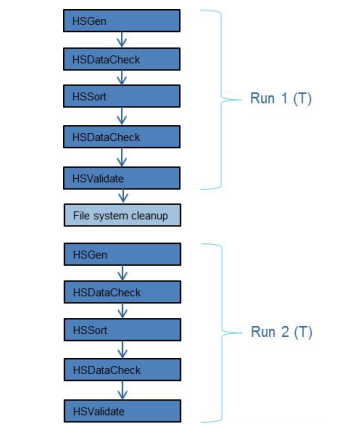
\includegraphics[width=5cm]{./Images/executionsTPC.png}
					\end{figure}

				\end{columns}
	
		\end{frame}
		
	\subsection*{Medida del rendimiento}	
			
		\begin{frame}{Rendimiento}
			Para hacer el análisis de la medida del rendimiento, TPCx-HS define las siguientes medidas:
			
			\color{ChetwodeBlue}\large Medida del rendimiento
			
			\color{ChetwodeBlue}\large Medida del rendimiento-precio.
		\end{frame}
				 